\documentclass[default]{beamer}
\setbeamertemplate{navigation symbols}{}

\usetheme{CambridgeUS}
%\useoutertheme{infolines}
\usecolortheme{beaver}

\usepackage[utf8]{inputenc}					% Выбор языка и кодировки
\usepackage[english, russian]{babel}	% Языки: русский, английский
\usepackage{csquotes}
\usepackage{tikz}
\usetikzlibrary{arrows,shapes,calc}
\usepackage{animate}
\usepackage{fp}
\usepackage{media9}
\usepackage{textpos}

\usepackage[
	language=auto,
	autolang=other,
	backend=biber,
	style=authortitle,
	sorting=ydnt,
	maxbibnames=5
]{biblatex}
\addbibresource{roboai_panov.bib}
				
\DeclareSourcemap{
	\maps[datatype=bibtex, overwrite]{
		\map{
			\step[fieldset=langid, fieldvalue=english]
			\step[fieldset=doi, null]
			\step[fieldset=issn, null]
			\step[fieldset=isbn, null]
			\step[fieldset=url, null]
			\step[fieldsource=language, fieldset=langid, origfieldval]
		}
	}
}
\DeclareBibliographyDriver{std}{%
	\usebibmacro{bibindex}%
	\usebibmacro{begentry}%
	\usebibmacro{author/editor+others/translator+others}%
	\setunit{\labelnamepunct}\newblock
	\usebibmacro{title}%
	\newunit\newblock
	\usebibmacro{maintitle+booktitle}
	\newunit\newblock
	\usebibmacro{journal}%
	\newunit\newblock
	\usebibmacro{date}%
	\newunit\newblock
	\usebibmacro{finentry}
}
\DeclareBibliographyAlias{article}{std}
\DeclareBibliographyAlias{book}{std}
\DeclareBibliographyAlias{inproceedings}{std}
\DeclareBibliographyAlias{incollection}{std}

\graphicspath{{../../images/}} 			% Пути к изображениям

\makeatletter
\setbeamertemplate{footline}
{
	\leavevmode%
	\hbox{%
		\begin{beamercolorbox}[wd=.333333\paperwidth,ht=2.25ex,dp=1ex,center]{author
				in head/foot}%
			\usebeamerfont{author in
				head/foot}\insertshortauthor~~\beamer@ifempty{\insertshortinstitute}{}{(\insertshortinstitute)}
		\end{beamercolorbox}%
		\begin{beamercolorbox}[wd=.333333\paperwidth,ht=2.25ex,dp=1ex,center]{title in
				head/foot}%
			\usebeamerfont{title in head/foot}\insertshorttitle
		\end{beamercolorbox}%
		\begin{beamercolorbox}[wd=.333333\paperwidth,ht=2.25ex,dp=1ex,right]{date in
				head/foot}%
			\usebeamerfont{date in head/foot}\insertshortdate{}\hspace*{1em}
			\insertframenumber{}\hspace*{2ex} 
		\end{beamercolorbox}
	}%
	\vskip0pt%
}

\addtobeamertemplate{frametitle}{}{
	\begin{textblock*}{100mm}(\textwidth-35pt,-20pt)
		
\includegraphics[width=1.5cm]{misc/logos/frccsc.png}
	\end{textblock*}
}

\newcommand{\predmatr}[3]{
	\node[ell, rectangle, minimum height = 15, minimum width = 7.5]  at (#1 pt,#2 pt) {}; 
	\node[ellf, rectangle, minimum height = 15, minimum width = 7.5] at (#1+7.5 pt,#2 pt) {};
	\node[minimum height = 15, minimum width = 15] (#3) at (#1+3.3pt,#2 pt) {};
	\draw[ell] (#1+7.5 pt,#2+7.5 pt) -- (#1 +7.5 pt,#2-7.5 pt);
}
\renewcommand*{\bibfont}{\tiny}
\setlength\bibitemsep{-5pt}

\begin{document}
	
	\title[Стратегическое управление]{Методы стратегического управления робототехнической системы в составе коалиции}
	\author[Панов]{Александр Панов}
	\institute[ФИЦ ИУ РАН]{Лаборатория динамических интеллектуальных систем\\Институт системного анализа\\ Федеральный исследовательский центр <<Информатика и управление>>\\Российской академии наук}
	\date[7 декабря]{7 декабря\\Семинар <<Интеллектуальные системы управления роботов>>} 
	
	\begin{frame}
		\titlepage
		\centering
		
\includegraphics[width=100pt]{misc/logos/ras.png} \hspace{10pt}
		
\includegraphics[width=80pt]{misc/logos/frccsc.png} \hspace{10pt}
		
\includegraphics[width=20pt]{misc/logos/hse.png}
	\end{frame}

	\section{Введение}
	\subsection{Стратегическое управление}
	\begin{frame}
		\frametitle{Когнитивные архитектуры}
		\begin{center}
			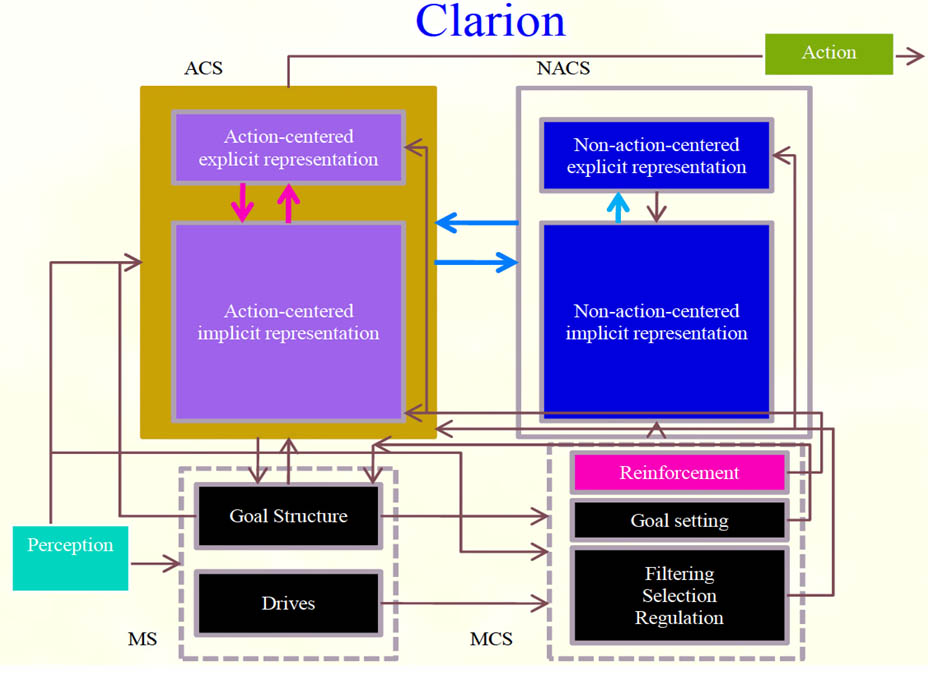
\includegraphics[width=0.3\textwidth]{agent-schemas/en/clarion.jpg}
			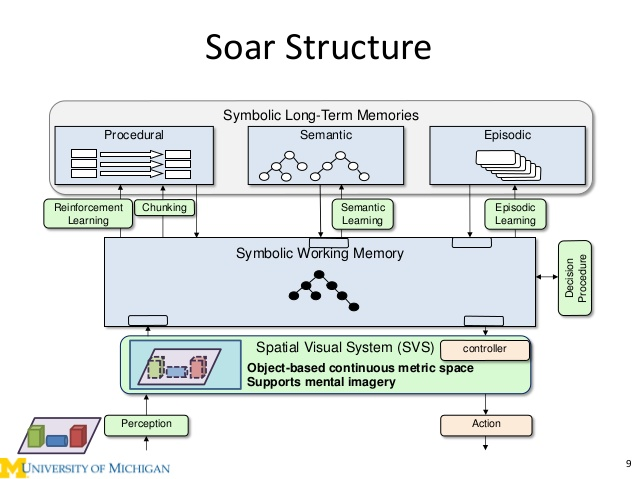
\includegraphics[width=0.3\textwidth]{agent-schemas/en/soar.jpg}
		\end{center}
		\scriptsize
		Недостатки современных когнитивных архитектур:
		\begin{itemize}
			\item Концептуальная нерешенность проблемы привязки символов (symbol grounding problem) - CLARION
			\item Отсутствие деятельностной модели поведения системы - реализация только некоторых когнитивных аспектов
			\item Иерархичность представления знаний (4D/RCS)
			\item Возможность реализации иерархического планирования
			\item Реализация обучения концептуальным знаниям - Cognitive Mario
			\item Моделирование рефлексивного поведения
		\end{itemize}
		\vspace{-5pt}
		\nocite{*}
		\printbibliography[keyword={symbgrnd}, resetnumbers=true]
	\end{frame}

	\subsection{Знаковая картина мира}
	
	\begin{frame}
		\frametitle{Картина мира субъекта деятельности}
		\scriptsize
		\onslide<1->{
			Картина мира субъекта деятельности - это представления субъекта о внешней среде, о своих собственных характеристиках, целях, мотивах, о других субъектах и операции (произвольные и непроизвольные), осуществляемые на основе этих представлений.
		}
		\onslide<2->{
			\par\smallskip
			Элементом картины мира является знак:
			\begin{itemize}
				\item в смысле культурно-исторического подхода Выготского-Лурии,
				\item выполняющий функции в соответствии с теорией деятельности Леонтьева.
			\end{itemize}
		}
		\onslide<3->{
			\begin{columns}
				\begin{column}{0.4\textwidth}
					\centering
					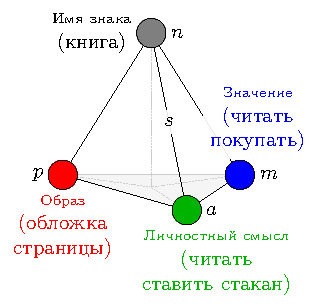
\includegraphics[width=0.6\textwidth]{signs/ru/sign_color_book_ru}
				\end{column}
		}
		\onslide<4->{
				\begin{column}{0.6\textwidth}
					\begin{columns}
						\begin{column}{0.5\textwidth}
							\centering
							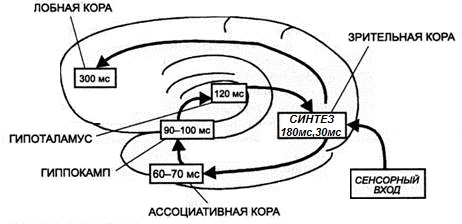
\includegraphics[width=\textwidth]{misc/phisio/ivan_cyrc}
						\end{column}
						\begin{column}{0.5\textwidth}
							\centering
							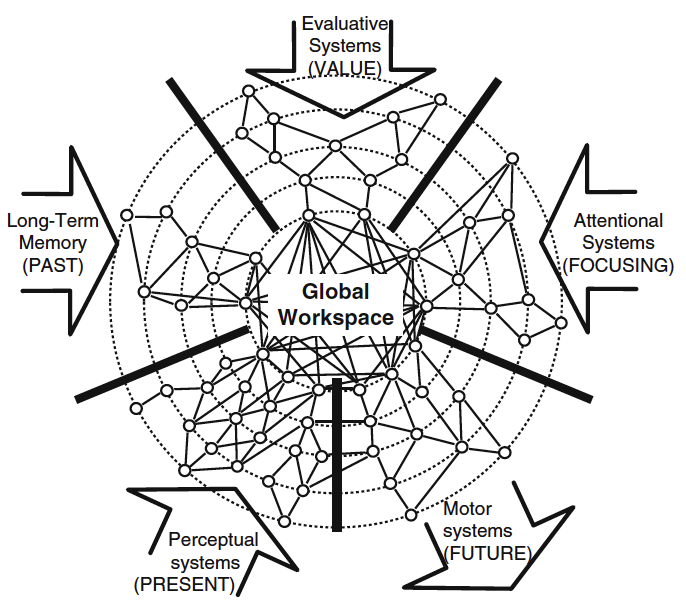
\includegraphics[width=\textwidth]{misc/phisio/workspace}
						\end{column}
					\end{columns}
					
				\end{column}
			\end{columns}
			В пользу существования такой структуры свидетельствуют:
			\begin{itemize}
				\item нейрофизиологические данные (Эдельман, Иваницкий, Маунткастл и др.),
				\item другие психологические теории (например, трехкомпонентная модель Станович).
			\end{itemize}
			\vspace{-5pt}
			\nocite{*}
			\printbibliography[keyword={sign}, resetnumbers=true]
		}
	\end{frame}

	\begin{frame}
		\frametitle{Уровни представления}
		\begin{figure}
			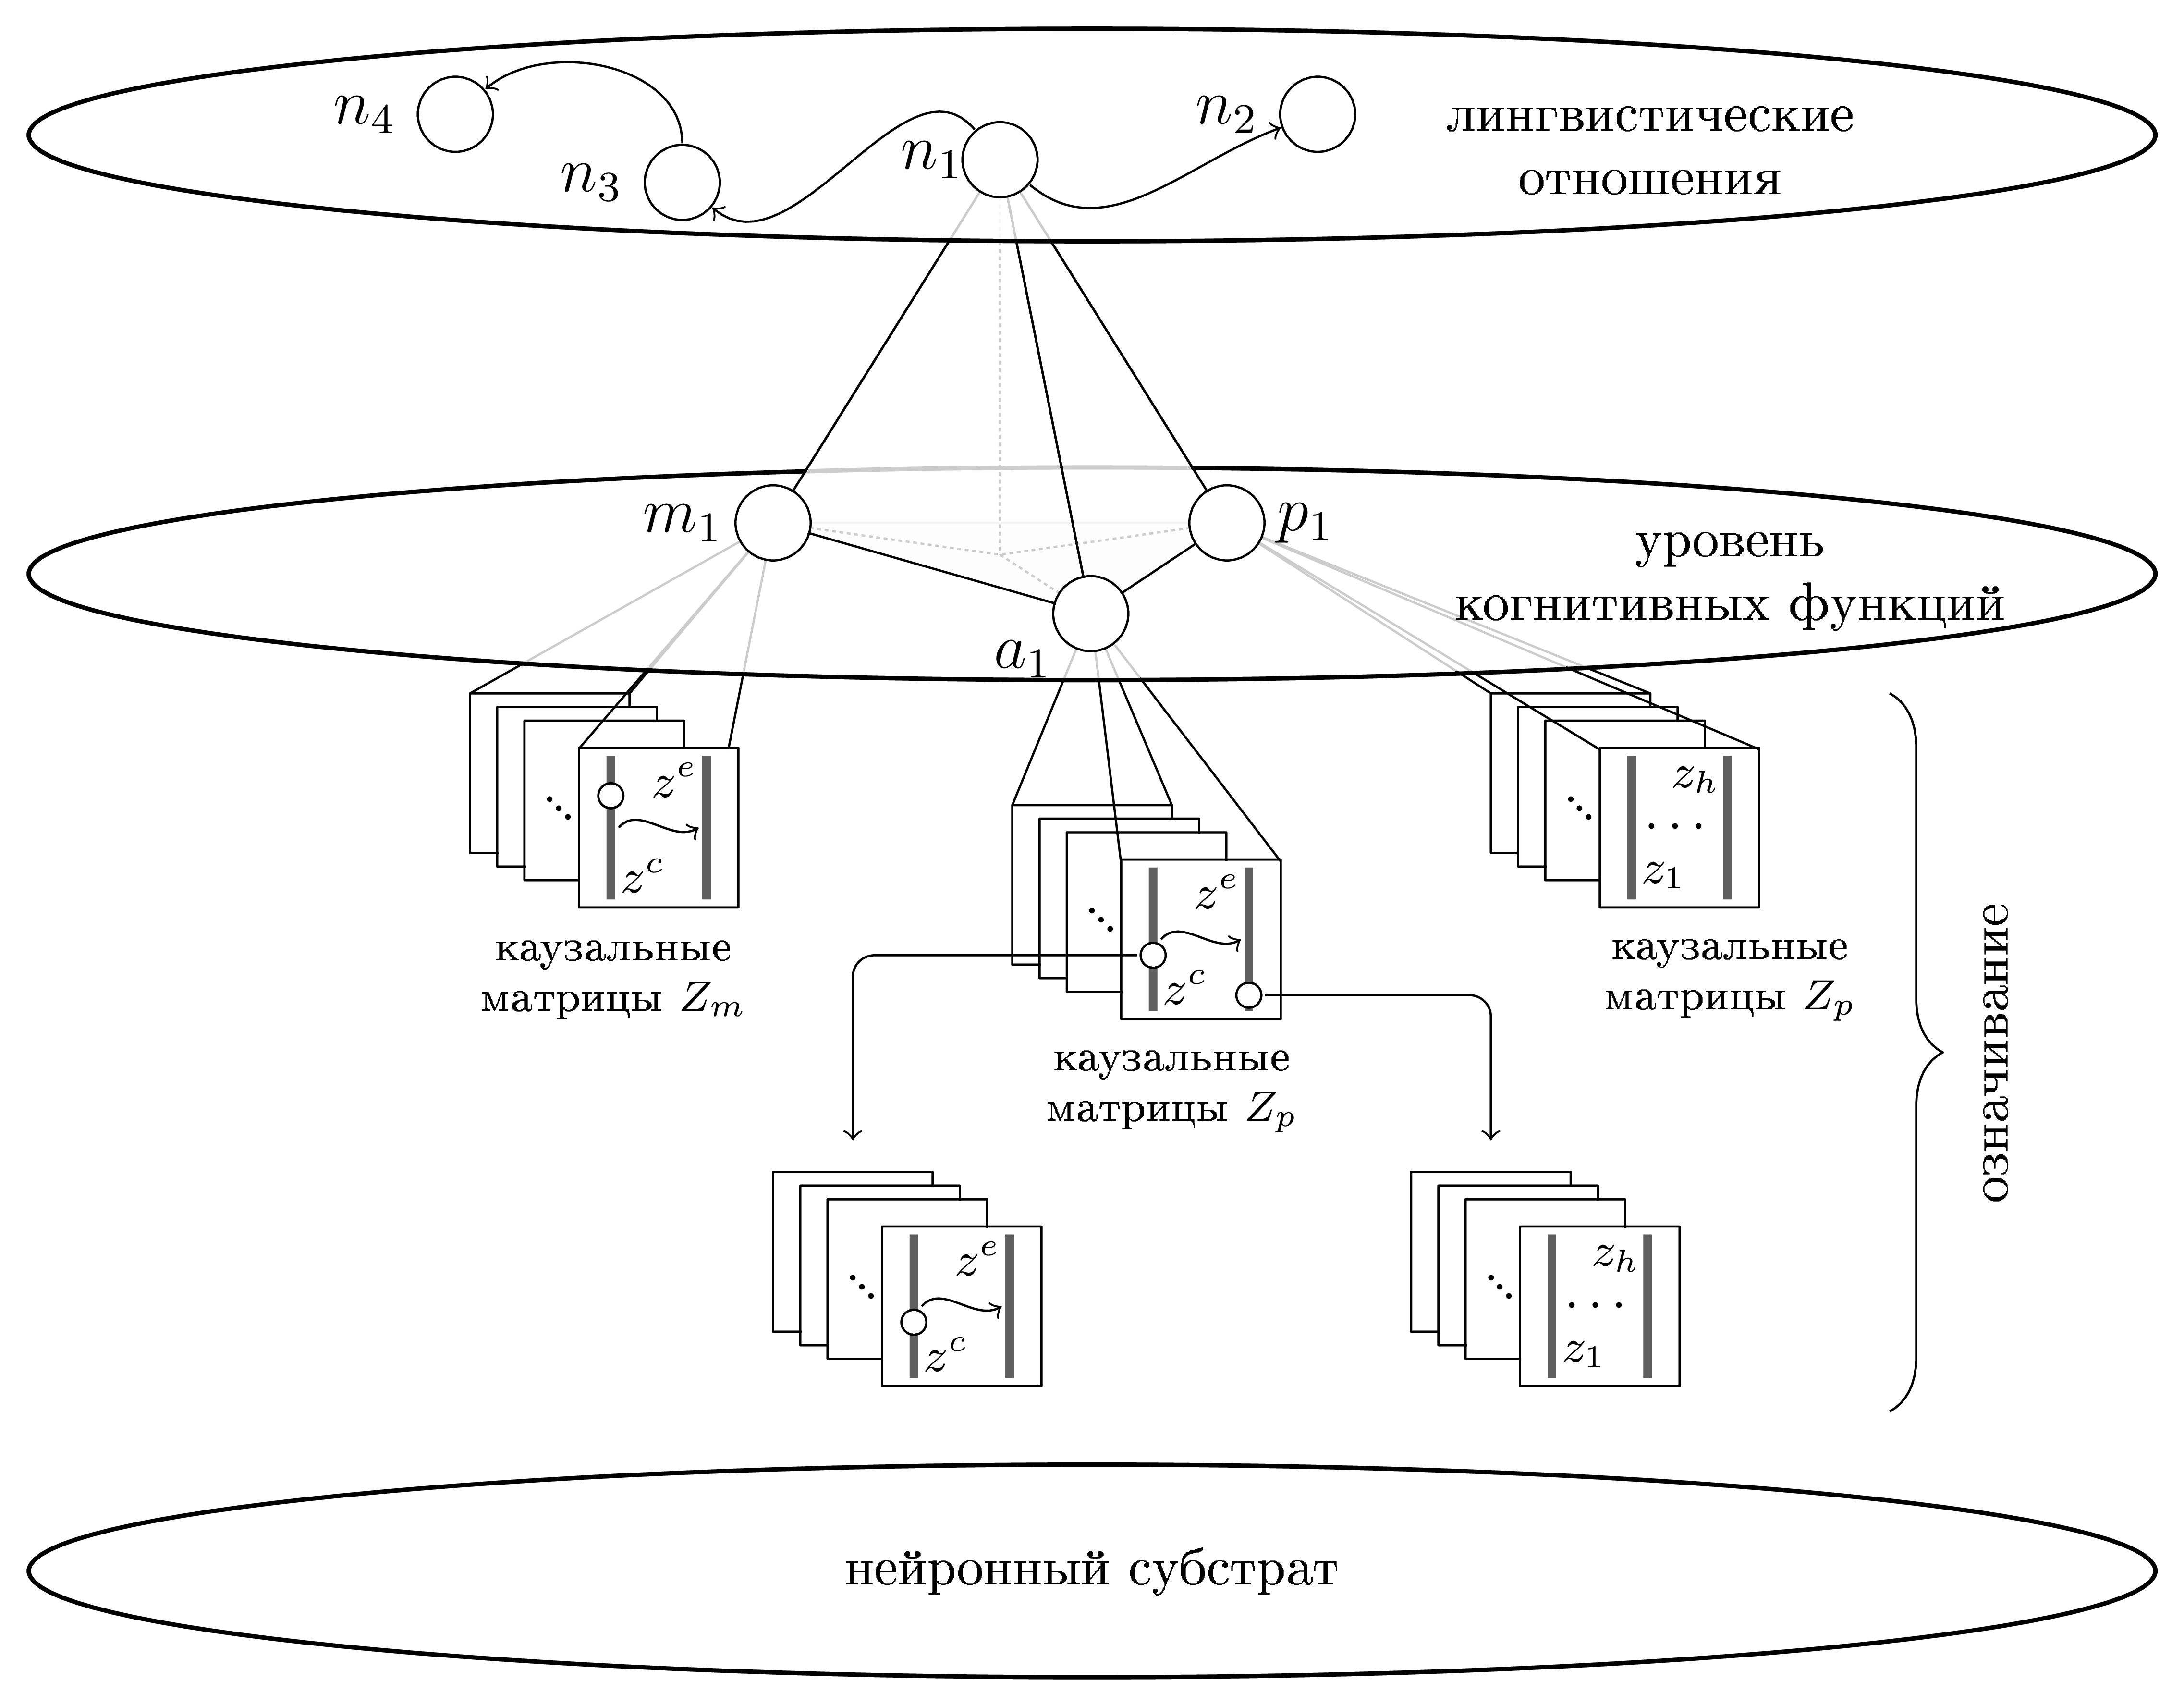
\includegraphics[width=0.7\textwidth]{signs/ru/sign_levels}
		\end{figure}
	\end{frame}

	\section{Модель элементов картины мира}
	
	\subsection{Образная компонента знака}
	\begin{frame}
		\frametitle{Каузальная матрица}                             
		\centering
		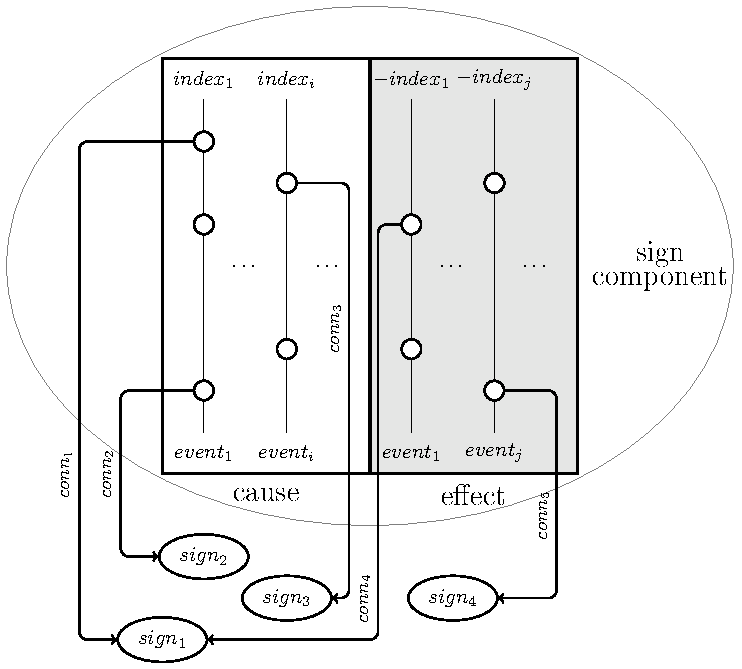
\includegraphics[width=0.7\textwidth]{causnet/caus_matr}
		\vspace{10pt}
		\nocite{*}
		\printbibliography[keyword={per}, resetnumbers=true]
	\end{frame}

	\begin{frame}
		\frametitle{Каузальная сеть на образах}
		\footnotesize
		\textbf{Каузальная сеть} на множестве образов знаков $W_p=\langle V_p, E_p \rangle$ - помеченный ориентированный граф, в котором
		\begin{itemize}
			\item каждому узлу $v\in V_p$ ставится в соответствие кортеж казуальных матриц $Z^p(s)$ образа некоторого знака $s$ ($v\rightarrow Z^p(s)$);
			\item ребро $e=(v_1, v_2)$ принадлежит множеству ребер графа $E$, если $v_1\rightarrow Z^p(s_1), v_2\rightarrow Z^p(s_2)$ и $s_1\in S_p(s_2)$;
			\item каждому ребру графа $e=(v_1, v_2), v_1\rightarrow Z^p(s_1), v_2\rightarrow Z^p(s_2)$ ставится в соответствие метка $\epsilon=(\epsilon_1,\epsilon_2,\epsilon_3)$ - кортеж трех натуральных чисел:
			\begin{itemize}
				\item $\epsilon_1$ - индекс исходной матрицы в кортеже $Z^p(s_1)$, может принимать специальное значение 0, если исходными могут служить любые матрицы из кортежа;
				\item $\epsilon_2$ - индекс целевой матрицы в кортеже $Z^p(s_2)$, строка которой ставится в соответствие признаку $s_1$;
				\item $\epsilon_2$ - индекс столбца в целевой матрице, в которой в соответствующей признаку $s_1$ строке стоит 1, может принимать положительные значения (\textit{столбцы условий}) и отрицательные (\textit{столбцы эффектов}).
			\end{itemize}		
		\end{itemize}
	\end{frame}

	\begin{frame}
		\frametitle{Каузальная сеть на образах: пример}
		
		\centering
		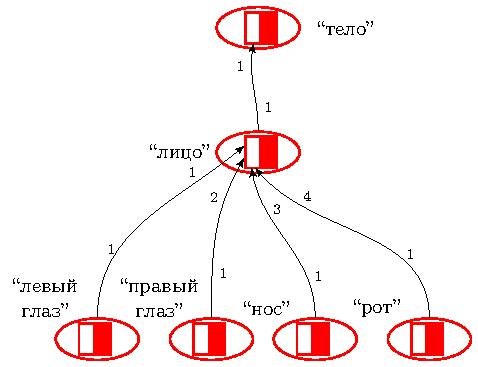
\includegraphics[page=1,width=0.6\textwidth]{examples/causnet/caus_net_colored}
		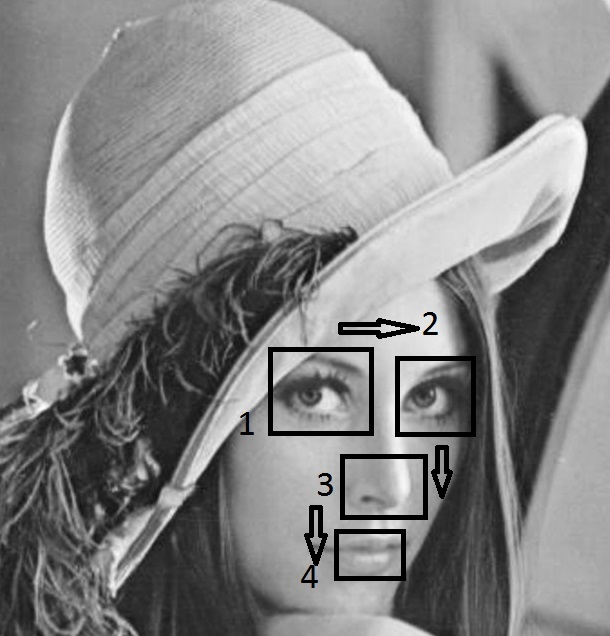
\includegraphics[width=0.4\textwidth]{misc/photos/face}
	
		\nocite{*}
		\printbibliography[keyword={signopernew}, resetnumbers=true]
	\end{frame}

	\begin{frame}
		\frametitle{Каузальная сеть на значениях: пример}
		
		\begin{figure}
			\includegraphics[page=2,width=0.7\textwidth]{examples/causnet/caus_net_colored}
		\end{figure}
		
	\end{frame}

	\begin{frame}
		\frametitle{Каузальная сеть на личностных смыслах: пример}
		
		\begin{figure}
			\includegraphics[page=3,width=0.7\textwidth]{examples/causnet/caus_net_colored}
		\end{figure}
		
	\end{frame}	

	\subsection{Семиотическая сеть}
	\begin{frame}
		\frametitle{Картина мира субъекта деятельности}
		
		\begin{columns}
			\begin{column}{0.55\textwidth}
				\begin{figure}
					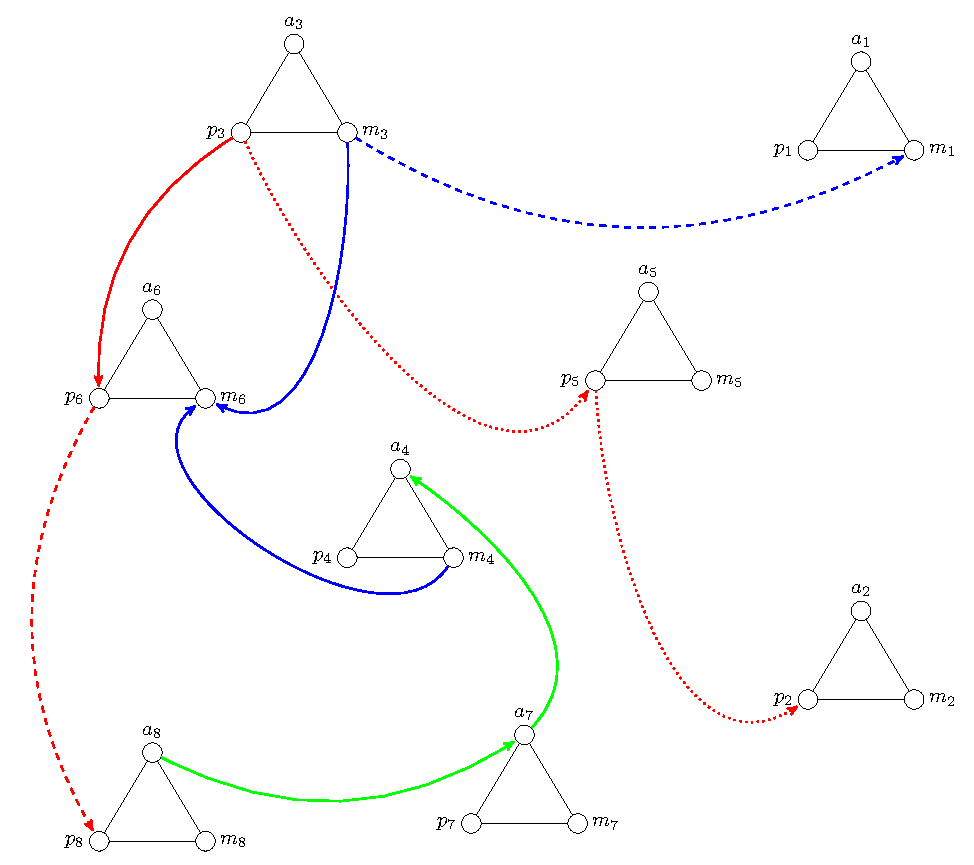
\includegraphics[width=\textwidth]{signnet/signs_net}
				\end{figure}
			\end{column}
			\begin{column}{0.45\textwidth}
				\textbf{Семиотическая сеть} - пятерка $\Omega=\langle W_p, W_m, W_a, R_n, \Theta \rangle$, где
				\begin{itemize}
					\item $W_p, W_m, W_a$ - соответственно каузальные сети на множестве образов, значений и личностных смыслах,
					\item $R_n$ - семейство отношений на множестве знаков, сгенерированных на основе трех каузальных сетей, т.е. $R_n=\{R_p, R_m, R_a\}$,
					\item $\Theta$ - семейство операций на множестве знаков.
				\end{itemize}
			\end{column}
		\end{columns}
		\nocite{*}
		\printbibliography[keyword={symbsign}, resetnumbers=true]
	\end{frame}	
	
	\section{Планирование поведения}
	\subsection{Схема алгоритма}
	\begin{frame}
		\frametitle{Алгоритм планирования поведения}
		
		\begin{columns}
			\begin{column}{0.6\textwidth}
				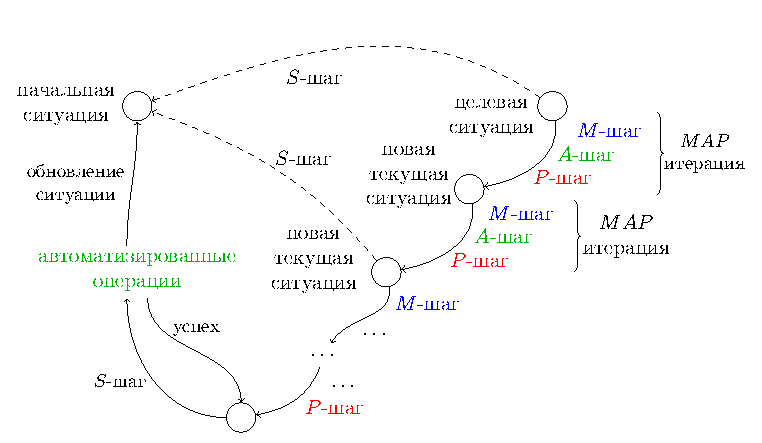
\includegraphics[width=\textwidth]{algo/ru/beh_plan2_ru}
				\vspace{10pt}
				\nocite{*}
				\printbibliography[keyword={plan}, resetnumbers=true]
				\printbibliography[keyword={causnet}]
			\end{column}
			\begin{column}{0.4\textwidth}
				\scriptsize
				Иерархический процесс планирования начинается с конченой ситуации и стремится достичь начальной ситуации.
				\par\bigskip
				MAP-итерация:
				\begin{itemize}
					\item \textit{S-step} -- поиск прецедентов выполнения действия в текущих условиях,
					\item \textit{M-step} -- поиск применимых действий на сети значений,
					\item \textit{A-step} -- генерация личностных смыслов, соответствующих найденным значениям,
					\item \textit{P-step} -- построение новой текущей ситуации по множеству признаков условий найденных действий.
					
				\end{itemize}
			\end{column}
		\end{columns}
		
	\end{frame}		
	
	\subsection{Примеры}
	\begin{frame}
		\frametitle{Пример: фрагмент сети на значениях}
		\begin{columns}
			\begin{column}{0.7\textwidth}
				\centering
				\includegraphics[page=2,width=\textwidth]{examples/plan/plan_nets}
			\end{column}
			\begin{column}{0.3\textwidth}
				\centering
				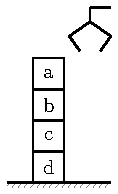
\includegraphics[page=1,width=\textwidth]{examples/plan/block_world}
			\end{column}
		\end{columns}
	\end{frame}	
	
	\begin{frame}
		\frametitle{Пример: сеть на смыслах - начальная ситуация}
		
		\centering
		\includegraphics[page=3,width=0.7\textwidth]{examples/plan/plan_nets}
		\par\bigskip
		\includegraphics[page=2,width=0.5\textwidth]{examples/plan/block_world}
		
		
	\end{frame}	
	
	\begin{frame}
		\frametitle{Пример: сеть на смыслах - целевая ситуация}
		\begin{columns}
			\begin{column}{0.7\textwidth}
				\centering
				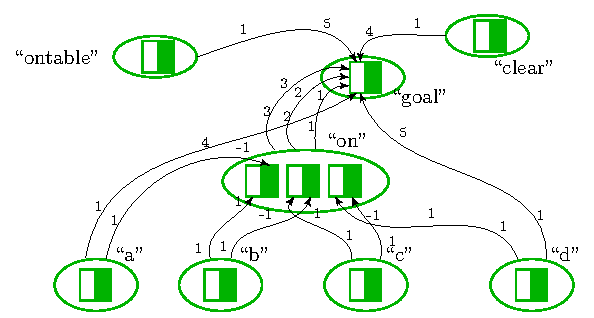
\includegraphics[page=1,width=\textwidth]{examples/plan/plan_nets}
			\end{column}
			\begin{column}{0.3\textwidth}
				\centering
				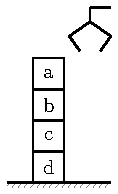
\includegraphics[page=1,width=\textwidth]{examples/plan/block_world}
			\end{column}
		\end{columns}
	\end{frame}	
	
	\begin{frame}
		\frametitle{Пример: фрагмент сети на значениях}
		\begin{columns}
			\begin{column}{0.7\textwidth}
				\centering
				\includegraphics[page=5,width=\textwidth]{examples/plan/plan_nets}
			\end{column}
			\begin{column}{0.3\textwidth}
				\centering
				\includegraphics[page=3,width=\textwidth]{examples/plan/block_world}
			\end{column}
		\end{columns}
	\end{frame}
	
	\begin{frame}
		\frametitle{Пример: генерация личностного смысла}
		
		\begin{tikzpicture}[overlay,remember picture,xshift=165pt,yshift=-50pt]
		\onslide<1->{
			\tikzstyle{ell}=[draw, thick, align=center, color=blue]
			\tikzstyle{ellf}=[draw, thick, align=center, color=blue, fill=blue]
			
			\node[ell, ellipse, minimum height = 30, minimum width = 100] (block) at (5 pt,0){};
			\predmatr{-30}{0}{block1}
			\predmatr{-10}{0}{block2}
			\predmatr{10}{0}{block3}	
			\predmatr{30}{0}{block4}
			\node at (35 pt, 20 pt) {``block''};
			
			\node[ell, ellipse, minimum height = 20, minimum width = 40] (c) at (32.5 pt, -50 pt){};
			\predmatr{30}{-50}{c1}
			\node at (10 pt, -35 pt) {``c''};		
			
			\node[ell, ellipse, minimum height = 20, minimum width = 40] (d) at (82.5 pt, -50 pt){};
			\predmatr{80}{-50}{d1}			
			\node at (60 pt, -35 pt) {``d''};	
			
			\node[ell, ellipse, minimum height = 20, minimum width = 40] (x) at (-37.5 pt, 50 pt){};
			\predmatr{-40}{50}{x1}
			\node at (-85 pt, 50 pt) {``block?x''};			
			
			\node[ell, ellipse, minimum height = 20, minimum width = 40] (y) at (42.5 pt, 50 pt){};
			\predmatr{40}{50}{y1}	
			\node at (85 pt, 50 pt) {``block?y''};
			
			\path[-latex'] (c.north) edge [out = 90, in = -80] node[above, black] {\scriptsize 1} node[above, black, near start] {\scriptsize 1} ([xshift=-3]block3.south);
			\path[-latex'] (d.north) edge [out = 90, in = -80] node[above, black, near end] {\scriptsize 1} node[above, black, near start] {\scriptsize 1} ([xshift=-3]block4.south);	
		}
		\onslide<1>{
			\node[ell, ellipse, minimum height = 20, minimum width = 40] (a) at (-77.5 pt, -50 pt){};
			\predmatr{-80}{-50}{a1}
			\node at (-100 pt, -35 pt) {``a''};
			
			\node[ell, ellipse, minimum height = 20, minimum width = 40] (b) at (-27.5 pt, -50 pt){};
			\predmatr{-30}{-50}{b1}
			\node at (-50 pt, -35 pt) {``b''};		
		}
		\onslide<1-2>{
			\path[-latex'] (a.north) edge [out = 90, in = -120] node[above, black, near end] {\scriptsize 1} node[above, black, near start] {\scriptsize 1} ([xshift=-3]block1.south);
			\path[-latex'] (b.north) edge [out = 90, in = -120] node[above, black, near end] {\scriptsize 1} node[above, black, near start] {\scriptsize 1} ([xshift=-3]block2.south);
		}			
		\onslide<1-3>{
			\path[-latex'] ([xshift=-10]block.north) edge [out = 90, in = -80] node[above, black] {\scriptsize 1} node[above, black, near start] {\scriptsize 0} ([xshift=-3]x1.south);
			\path[-latex'] ([xshift=10]block.north) edge [out = 90, in = -100] node[above, black] {\scriptsize 1} node[above, black, near start] {\scriptsize 0} ([xshift=-3]y1.south);
		}
		\onslide<1-4>{
			\node[ell, ellipse, minimum height = 20, minimum width = 40] (unstack) at (2.5 pt, 100 pt){};
			\predmatr{0}{100}{unstack1}
			\node at (-15 pt, 120 pt) {``unstack''};
			
			\node[ell, ellipse, minimum height = 20, minimum width = 40] (on) at (-77.5 pt, 100 pt){};
			\predmatr{-80}{100}{on1}
			\node at (-115 pt, 100 pt) {``on''};
			
			\path[-latex'] (x.north) edge [out = 90, in = -100] node[above, black, near end] {\scriptsize -1} node[above, black, near start] {\scriptsize 1} ([xshift=2]unstack1.south);
			\path[-latex'] (y.north) edge [out = 90, in = -80] node[above, black, near end] {\scriptsize -2} node[above, black, near start] {\scriptsize 1} ([xshift=5]unstack1.south);
			\path[-latex'] (on.east) edge [out = 0, in = 180] node[above, black, near end] {\scriptsize 1} node[above, black, near start] {\scriptsize 1} ([yshift=-3]unstack1.west);
			
			\path[-latex'] ([xshift=-10]x.north) edge [out = 100, in = -140] node[above, black] {\scriptsize 1} node[above, black, very near start] {\scriptsize 1} ([xshift=-3]on1.south);	
			\path[-latex'] ([xshift=-10]y.north) edge [out = 150, in = -30] node[above, black, near end] {\scriptsize -1} node[above, black, very near start] {\scriptsize 1} ([xshift=3]on1.south);					
		}			
		\onslide<1-5>{
			\node[ell, ellipse, minimum height = 20, minimum width = 40] (holding) at (82.5 pt, 120 pt){};
			\predmatr{80}{120}{holding1}
			\node at (125 pt, 120 pt) {``holding''};
			
			\node[ell, ellipse, minimum height = 20, minimum width = 40] (clear) at (82.5 pt, 90 pt){};
			\predmatr{80}{90}{clear1}
			\node at (120 pt, 90 pt) {``clear''};
			
			\path[-latex'] (clear.west) edge [out = 180, in = 0] node[above, black, near end] {\scriptsize -2} node[above, black, near start] {\scriptsize 1} ([yshift=-3]unstack1.east);
			\path[-latex'] (holding.west) edge [out = 180, in = 0] node[above, black, near end] {\scriptsize -1} node[above, black, near start] {\scriptsize 1} ([yshift=3]unstack1.east);
			
		}
		\onslide<2->{
			\tikzstyle{ell}=[draw, thick, align=center, color=green!70!black]
			\tikzstyle{ellf}=[draw, thick, align=center, color=green!70!black, fill=green!70!black]
			
			\node[ell, ellipse, minimum height = 20, minimum width = 40] (a) at (-77.5 pt, -50 pt){};
			\predmatr{-80}{-50}{a1}
			\node at (-100 pt, -35 pt) {``a''};
			
			\node[ell, ellipse, minimum height = 20, minimum width = 40] (b) at (-27.5 pt, -50 pt){};
			\predmatr{-30}{-50}{b1}
			\node at (-50 pt, -35 pt) {``b''};
		}
		\onslide<3->{
			\path[-latex', very thick] (a.north) edge [out = 90, in = -120] node[above, black, near end] {\scriptsize 1} node[above, black, near start] {\scriptsize 1} ([xshift=-3]block1.south);
			\path[-latex', very thick] (b.north) edge [out = 90, in = -120] node[above, black, near end] {\scriptsize 1} node[above, black, near start] {\scriptsize 1} ([xshift=-3]block2.south);	
		}
		\onslide<4->{
			\path[-latex', very thick] ([xshift=-10]block.north) edge [out = 90, in = -80] node[above, black] {\scriptsize 1} node[above, black, near start] {\scriptsize 0} ([xshift=-3]x1.south);
			\path[-latex', very thick] ([xshift=10]block.north) edge [out = 90, in = -100] node[above, black] {\scriptsize 1} node[above, black, near start] {\scriptsize 0} ([xshift=-3]y1.south);
		}
		\onslide<5->{
			\node[ell, ellipse, minimum height = 20, minimum width = 40] (unstack) at (2.5 pt, 100 pt){};
			\predmatr{0}{100}{unstack1}
			\node at (-15 pt, 120 pt) {``unstack''};
			
			\node[ell, ellipse, minimum height = 20, minimum width = 40] (on) at (-77.5 pt, 100 pt){};
			\predmatr{-80}{100}{on1}
			\node at (-115 pt, 100 pt) {``on''};
			
			\path[-latex', very thick] (on.east) edge [out = 0, in = 180] node[above, black, near end] {\scriptsize 1} node[above, black, near start] {\scriptsize 1} ([yshift=-3]unstack1.west);
			
			\path[-latex', very thick] ([xshift=-10]x.north) edge [out = 100, in = -140] node[above, black] {\scriptsize 1} node[above, black, very near start] {\scriptsize 1} ([xshift=-3]on1.south);	
			\path[-latex', very thick] ([xshift=-10]y.north) edge [out = 150, in = -30] node[above, black, near end] {\scriptsize -1} node[above, black, very near start] {\scriptsize 1} ([xshift=3]on1.south);
			\path[-latex', very thick] (x.north) edge [out = 90, in = -100] node[above, black, near end] {\scriptsize -1} node[above, black, near start] {\scriptsize 1} ([xshift=2]unstack1.south);
			\path[-latex', very thick] (y.north) edge [out = 90, in = -80] node[above, black, near end] {\scriptsize -2} node[above, black, near start] {\scriptsize 1} ([xshift=5]unstack1.south);	
		}
		\onslide<6->{
			\node[ell, ellipse, minimum height = 20, minimum width = 40] (holding) at (82.5 pt, 120 pt){};
			\predmatr{80}{120}{holding1}
			\node at (125 pt, 120 pt) {``holding''};
			
			\node[ell, ellipse, minimum height = 20, minimum width = 40] (clear) at (82.5 pt, 90 pt){};
			\predmatr{80}{90}{clear1}
			\node at (120 pt, 90 pt) {``clear''};
			
			\path[-latex', very thick] (clear.west) edge [out = 180, in = 0] node[above, black, near end] {\scriptsize -2} node[above, black, near start] {\scriptsize 1} ([yshift=-3]unstack1.east);
			\path[-latex', very thick] (holding.west) edge [out = 180, in = 0] node[above, black, near end] {\scriptsize -1} node[above, black, near start] {\scriptsize 1} ([yshift=3]unstack1.east);
		}			
		\end{tikzpicture}
	\end{frame}
	
	\begin{frame}
		\frametitle{Пример: текущая ситуация}
		\begin{columns}
			\begin{column}{0.7\textwidth}
				\centering
				\includegraphics[page=4,width=\textwidth]{examples/plan/plan_nets}
			\end{column}
			\begin{column}{0.3\textwidth}
				\centering
				\includegraphics[page=3,width=\textwidth]{examples/plan/block_world}
			\end{column}
		\end{columns}
	\end{frame}

	\begin{frame}
		\frametitle{Обучение в процессе планирования}
		
		Образование нового правила и сохранение ситуаций - образование новых каузальных матриц
		\par\bigskip
		\centering
		\includegraphics[page=6,width=0.6\textwidth]{examples/plan/plan_nets}
		\includegraphics[page=7,width=0.4\textwidth]{examples/plan/plan_nets}
	\end{frame}

	\begin{frame}
		\frametitle{Реализация на реальном роботе}

		\centering
		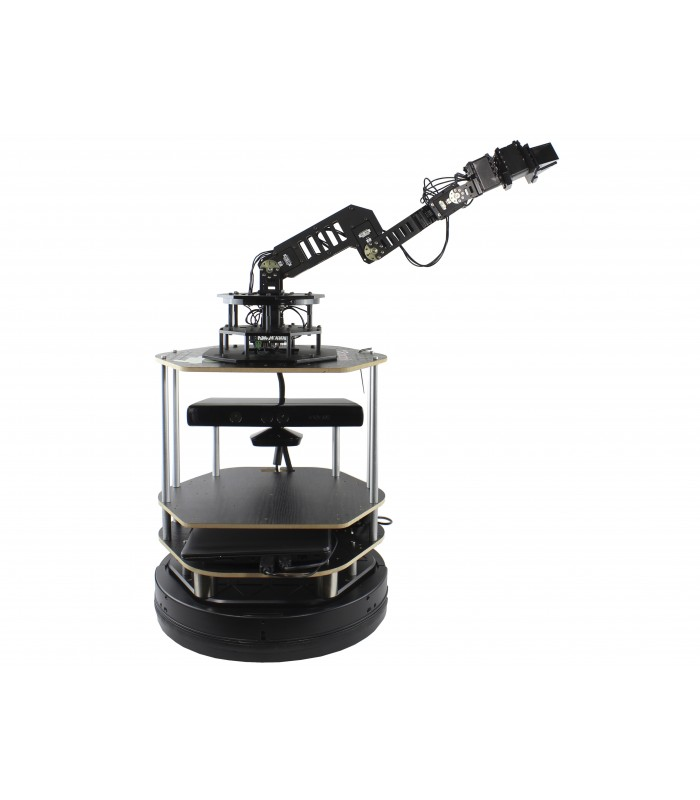
\includegraphics[width=0.7\textheight]{misc/agents/turtlebot-2.jpg}
	\end{frame}

	\begin{frame}
		\frametitle{Этап целеполагания}
		\begin{center}
			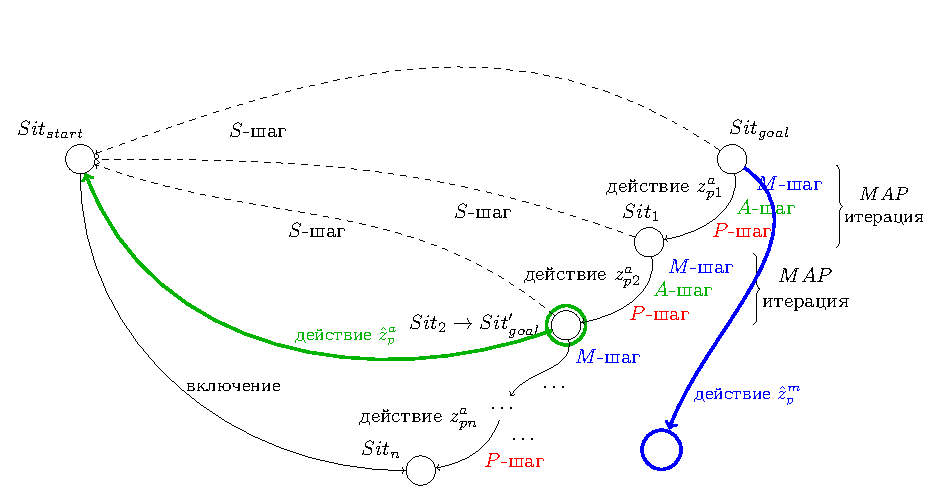
\includegraphics[width=0.8\textwidth]{algo/ru/gmap_ru}
		\end{center}
		\nocite{*}
		\printbibliography[keyword={goalres}, resetnumbers=true]
	\end{frame}

	\section{Прикладные задачи}
	\subsection{Многоагентная постановка}
	\begin{frame}
		\frametitle{Особенности постановки задачи}
		
		Рассматривается случай группового взаимодействия автономных технических объектов (агентов), в котором:
		\begin{itemize}
			\item агенты решают общую задачу (имеют общую цель высшего уровня),
			\item агенты действуют независимо друг от друга (децентрализованное управление), в т.ч. могут ставить индивидуальные подцели и достигать их,
			\item агенты обладают различными характеристиками, как техническими, так и когнитивными, т.е. разными стратегиями поведения,
			\item агенты обладают различными картинами мира,
			\item агенты действуют в меняющейся среде.
		\end{itemize}
		
	\end{frame}
	
	\begin{frame}
		\frametitle{Требования к представлению знаний}
		
		На представление пространственных и временных знаний в задаче согласованного перемещения с такими особенностями налагается ряд ограничений:
		\begin{itemize}
			\item необходимость поддержки некоторого протокола коммуникации, разделение знаний на коммуницируемые и некоммуницируемые (личные),
			\item необходимость выделения компоненты знания, не зависящей от индивидуальных (личных) характеристик агента,
			\item требование к наличию механизма связывания реальных объектов внешней среды и процедур их распознавания с символьным коммуницируемым представлением (symbol grounding problem),
			\item поддержка механизмов пополнения картины мира (обучение и абстрагирование).
		\end{itemize}
	\end{frame}

	\begin{frame}
		\frametitle{Практические задачи}
		
		\centering
		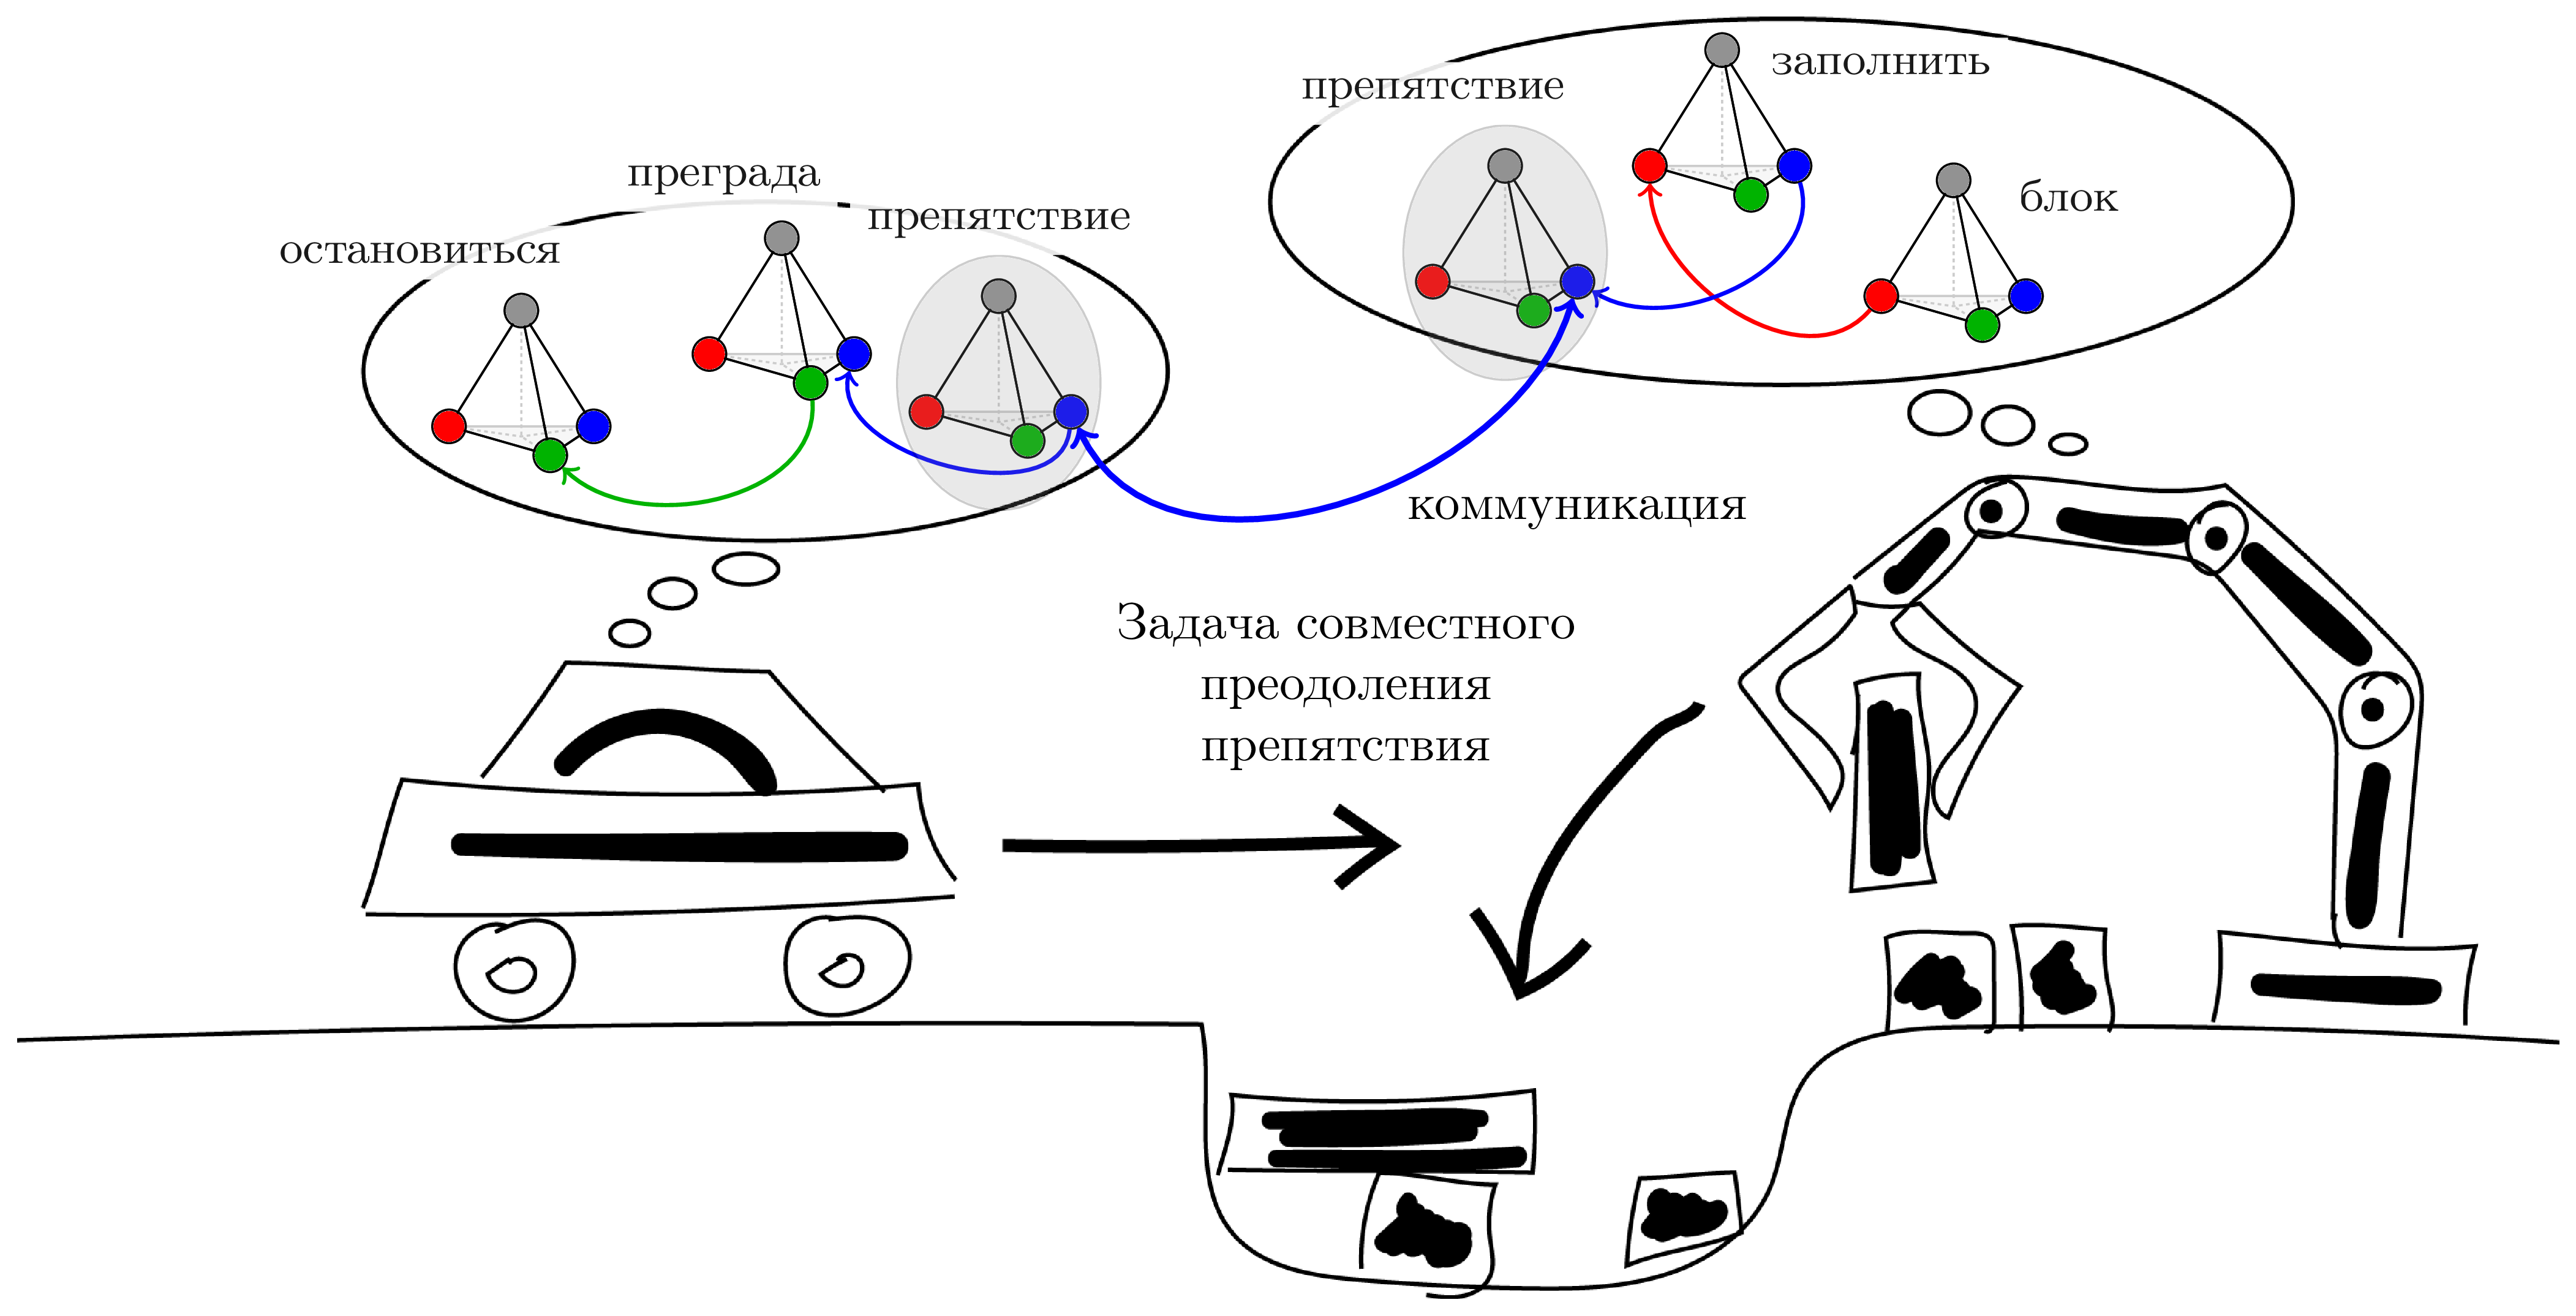
\includegraphics[width=\textwidth]{examples/signs/robotic_signs}

	\end{frame}
	
	\subsection{Задача интеллектуального перемещения}
	\begin{frame}
		\frametitle{Задача интеллектуального перемещения}
		
		\begin{columns}
			\begin{column}{0.55\textwidth}
				\begin{center}
					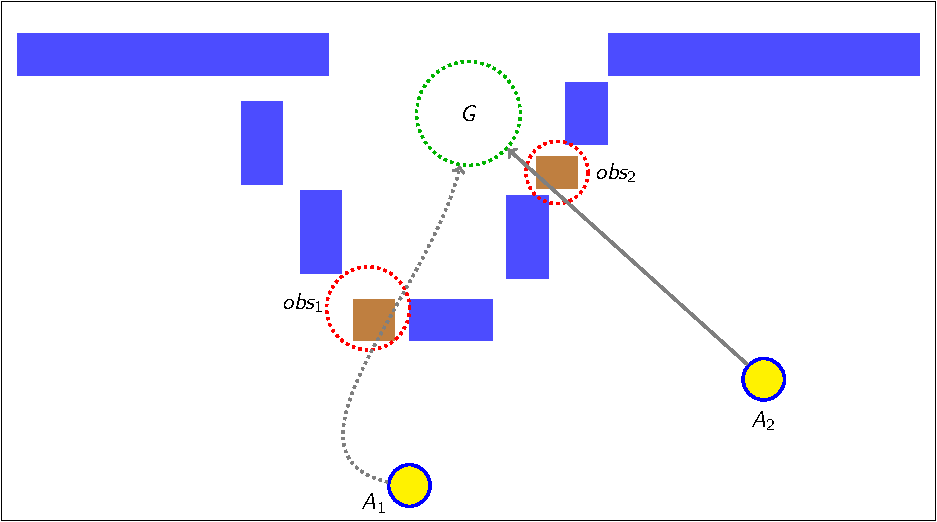
\includegraphics[page=1,width=0.8\textwidth]{examples/plan/slides_colored}
				\end{center}
				\vspace{-7pt}
				\small
				\textbf{Задача}
				
				Целевая область не достижима некоторым агентом самостоятельно (с использованием только методов планирования траектории).
				
				\textbf{Решение}
				
				Агенты должны поддерживать коммуникацию и модифицировать свои собственные планы с учетом коалиционных подзадач.
				
			\end{column}
			\begin{column}{0.45\textwidth}
				Особенности:
				\begin{itemize}
					\item Меняющаяся внешняя среда.
					\item Различные типы препятствий (некоторые могут быть разрушены).
					\item Агенты обладают различной функциональностью.
					\item Общая пространственная цель (ВСЕ агенты должны достичь определенной области на карте).
				\end{itemize}
			\end{column}
		\end{columns}
	\end{frame}
	
	\begin{frame}
		\frametitle{Представление пространственных знаний}
		
		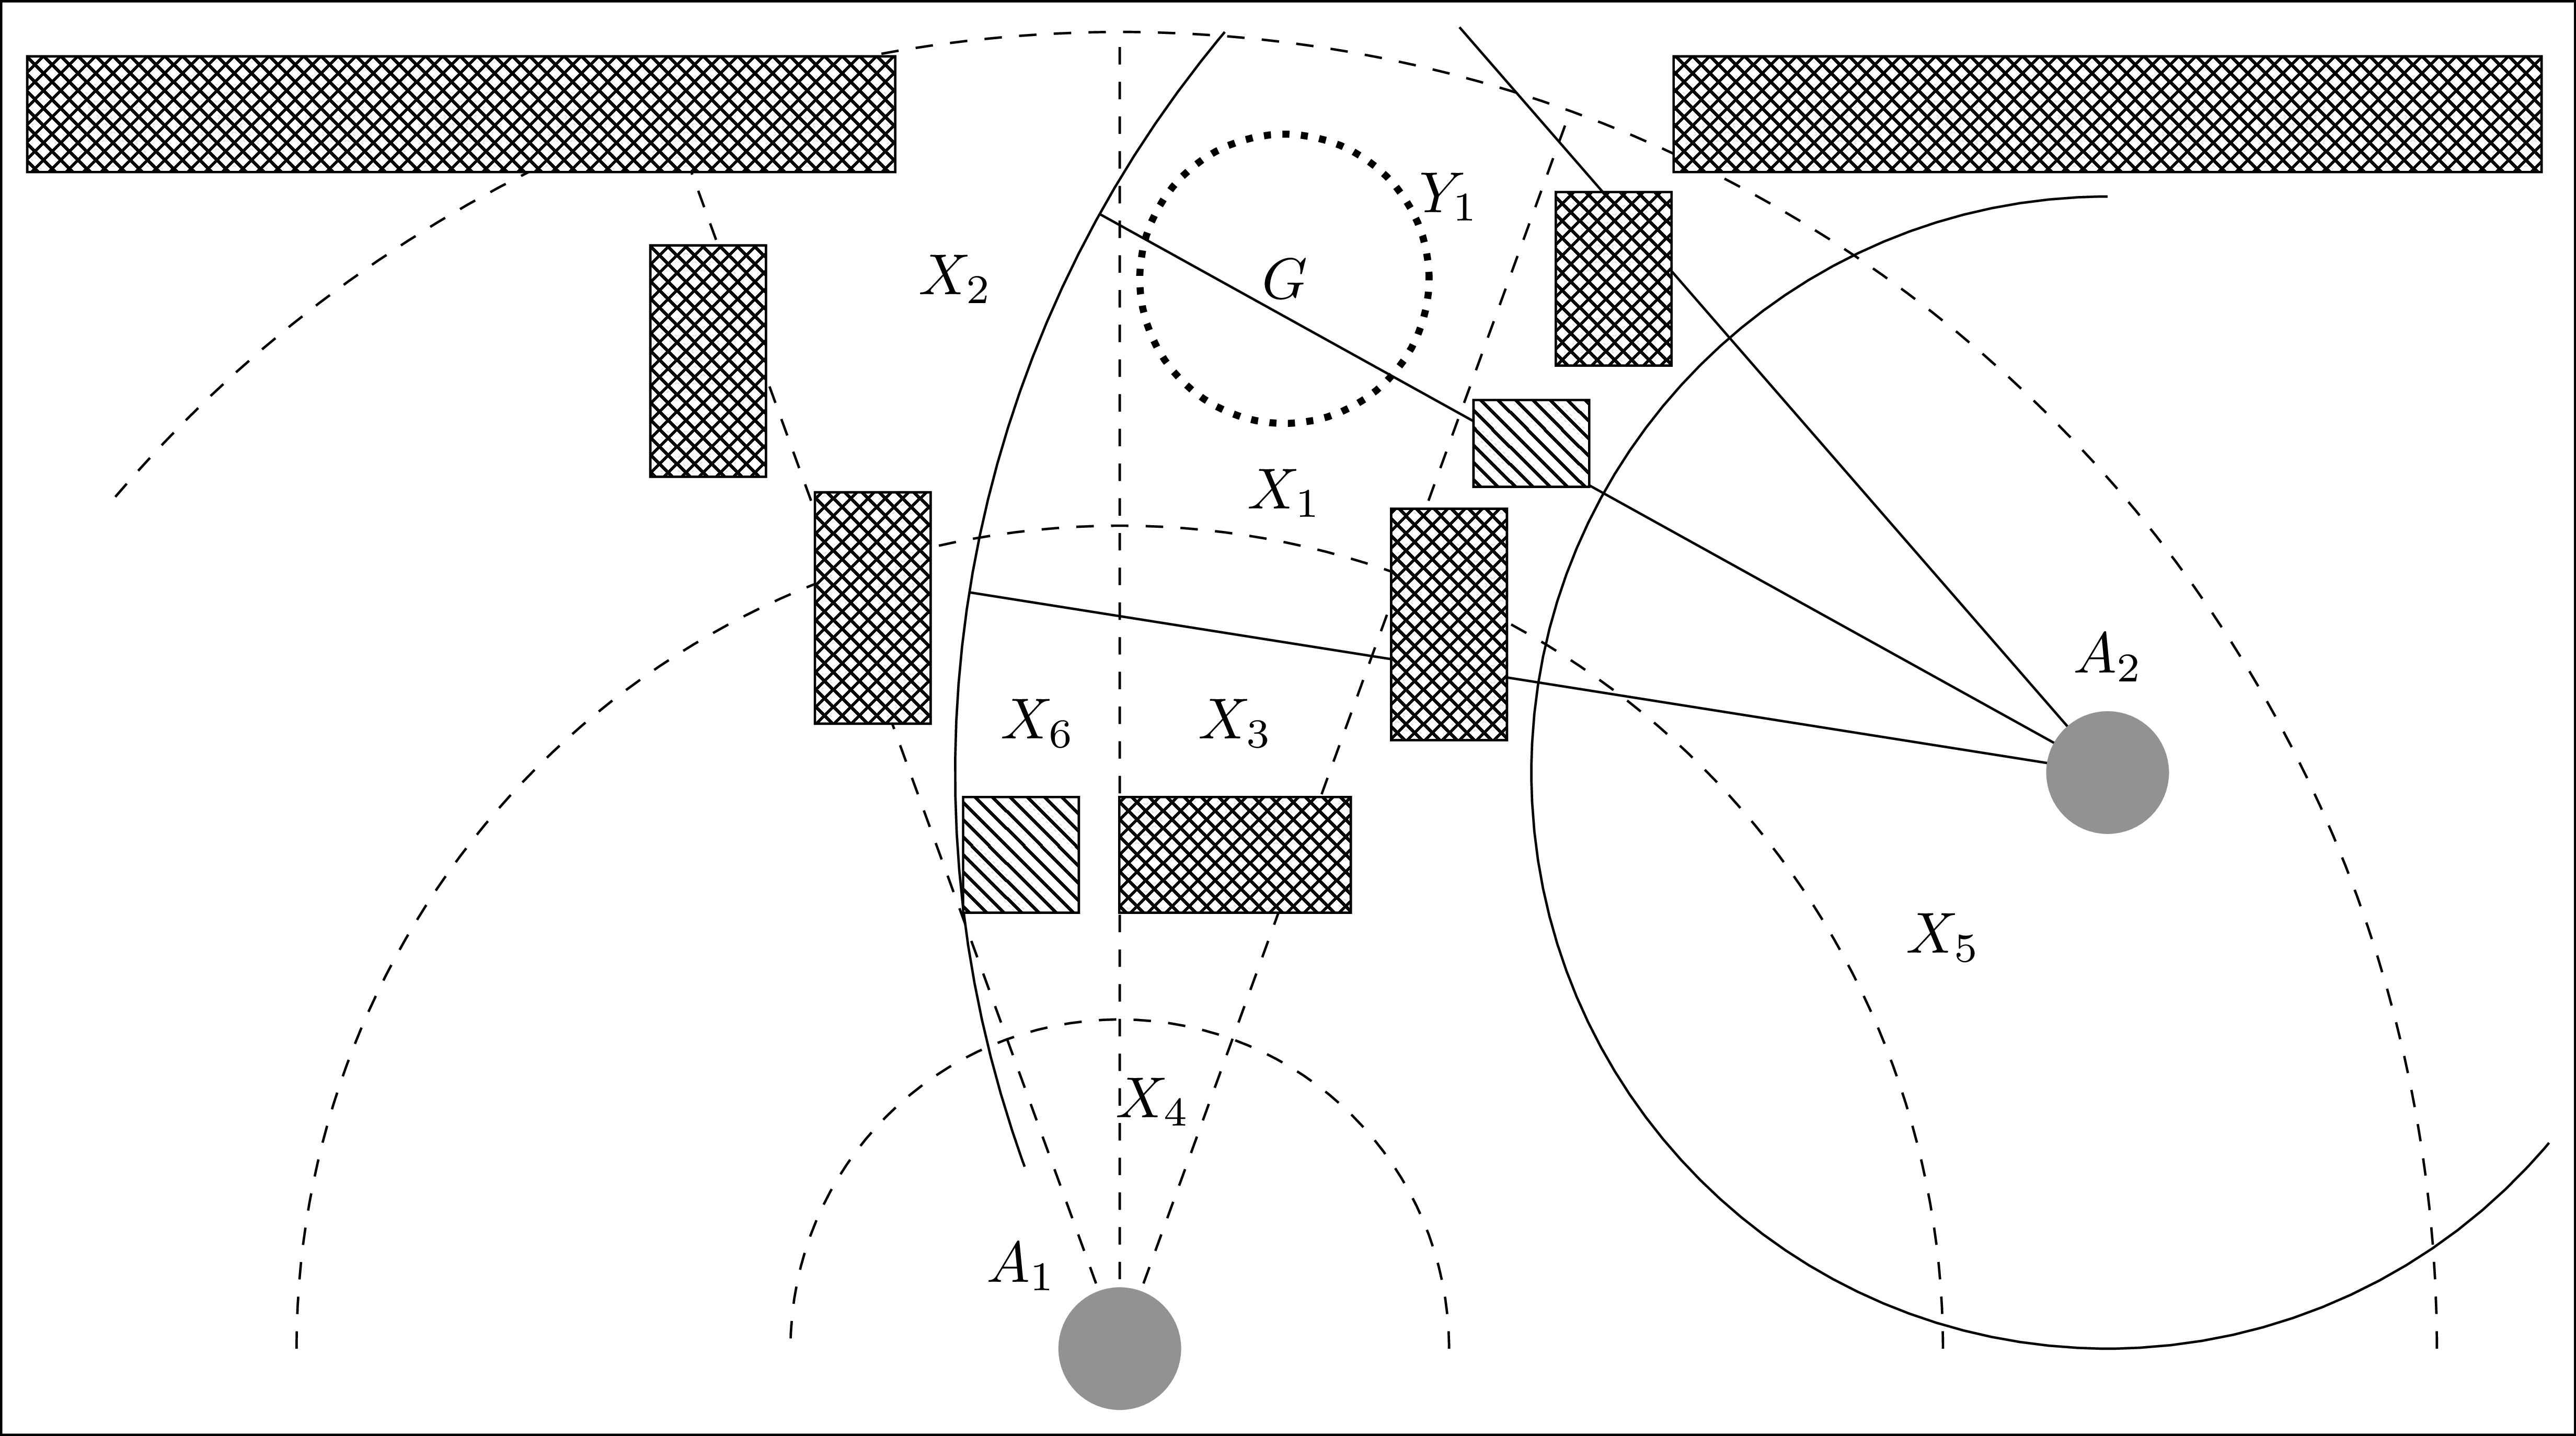
\includegraphics[width=\textwidth]{examples/representations/rita_ex_proc.png}
		
		\nocite{*}
		\printbibliography[keyword={planknow}, resetnumbers=true]
	\end{frame}

	\begin{frame}
		\frametitle{Представление пространственных знаний}
		
		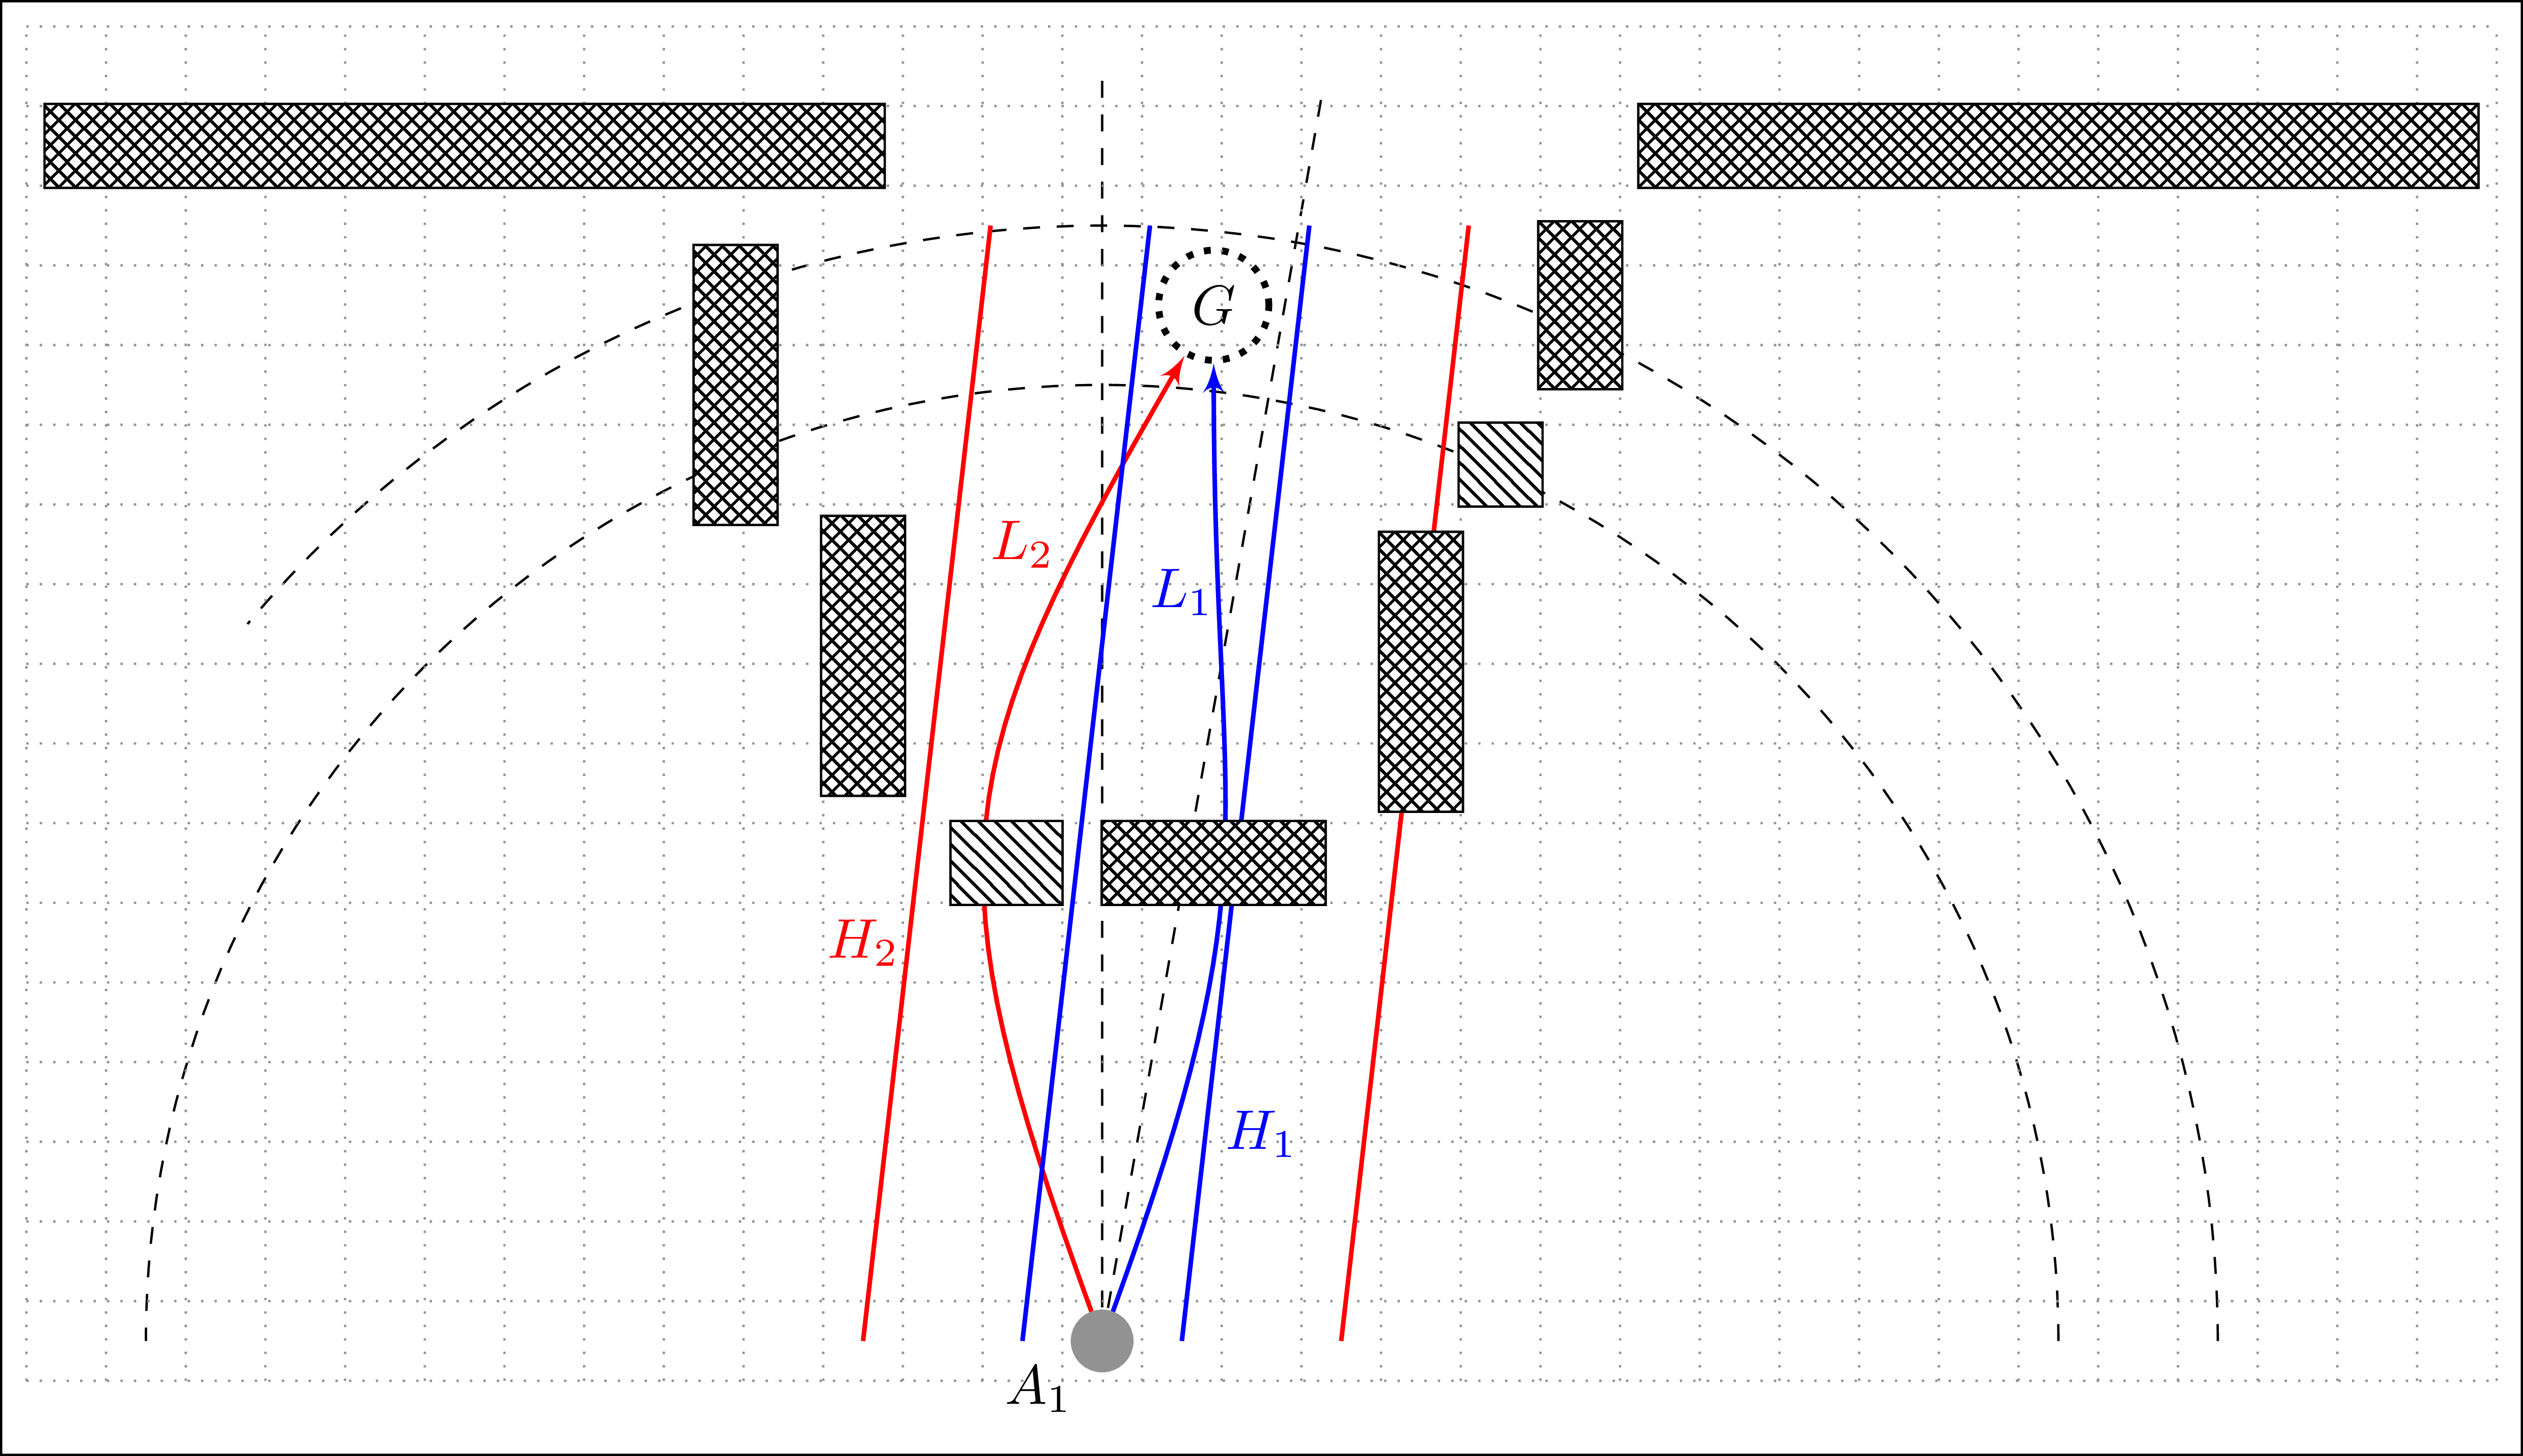
\includegraphics[width=\textwidth]{examples/representations/bica_psy_path.png}
		
		\nocite{*}
		\printbibliography[keyword={behplanrus}, resetnumbers=true]
	\end{frame}	
	\begin{frame}
		\frametitle{Представление действий по перемещению}
		
		Действия по перемещению "--- знаки $s_t$ (признаки $f_t$, $t$ "--- тип перемещения), которым соответствуют каузальные матрицы типа $Z_t$, состоящие из трёх столбцов 
		\[
		z_1=(l_x, I), z_2=(l_y, d_u, E), z_3=(l_y, I, t_v),
		\]
		где 
		\begin{itemize}
			\item $l_x$, $l_y$ "--- признаки, соответствующие категории расстояния в пространственной логике  (например, вплотную, близко, далеко и др.), 
			\item $d_u$ "--- признак, соответствующий категории направления в пространственной логике (например, впереди, слева и др.), 
			\item $t_v$ "--- признак, соответствующий категории времени во временной логике (например, скоро, в будущем и др.),
			\item $I$ "--- признак присутствия самого агента, 
			\item $E$ "--- признак отсутствия препятствия.
		\end{itemize}
	\end{frame}	

	\begin{frame}
		\frametitle{Реализация в симуляционной среде}
		
		\centering
		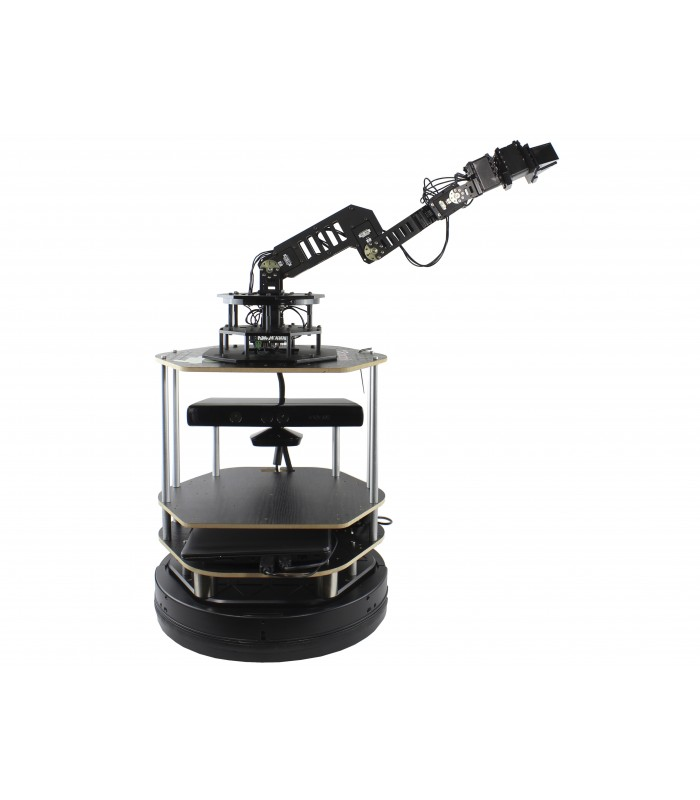
\includegraphics[width=0.7\textheight]{misc/agents/turtlebot-2.jpg}
	\end{frame}
	
	\begin{frame}
		\frametitle{Распределение ролей при решении задачи}
		\begin{center}
			\scalebox{0.7}{
				\animategraphics{12}{examples/plan/slides_colored}{}{}			
			}
		\end{center}
	\end{frame}
	
	\subsection{Распределение ролей в коллективе}
	\begin{frame}
		\frametitle{Знаки Я и Они в алгоритме планирования MAP}
		
		\begin{center}
			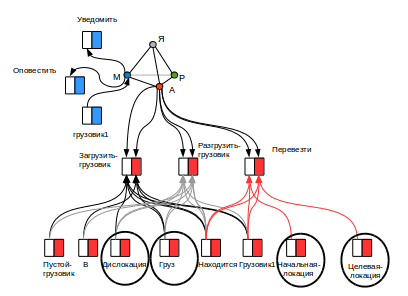
\includegraphics[width=0.6\textwidth]{sign-schemas/I-sign.png}
			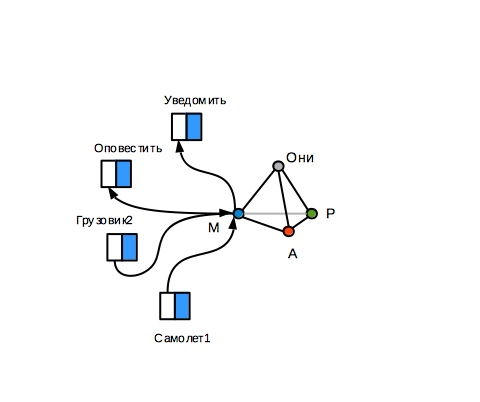
\includegraphics[width=0.5\textwidth]{sign-schemas/they-sign.png}
		\end{center}
	
		Составление плана вида $P(Ak)=\langle a_1(A_{i1}), a_2(A_{i2}),\dots\rangle$.
		\nocite{*}
		\printbibliography[keyword={roledistrib}, resetnumbers=true]
	\end{frame}

	\begin{frame}
		\frametitle{Коллективное планирование}
		\small
		Особенности алгоритма коллективного планирования:
		\begin{itemize}
			\item этап означивания, 
			\item этап индивидуального планирования, 
			\item этап согласования планов и 
			\item этап сохранения опыта.
		\end{itemize}
		
		Экспериментальное исследование:
		\begin{itemize}
			\item три агента планирования, каждый из которых может взаимодействовать с двумя видами блоков, всего используется три вида блоков, в количестве двух блоков каждого вида;
			\item использование опыта построения планов агентами из эксперимента 1 при повторном решении задачи эксперимента 1;
			\item задача эксперимента 1 расширяется с помощью добавления двух больших блоков в вершину башни;
			\item задача перемещения двумя грузовиками разной грузоподъемности четырёх различных грузов в аэропорт.
		\end{itemize}
	\end{frame}

	\subsection{Обучение с подкреплением}
	\begin{frame}
		\frametitle{Формирование элементов картины мира}
		\footnotesize
		\centering
		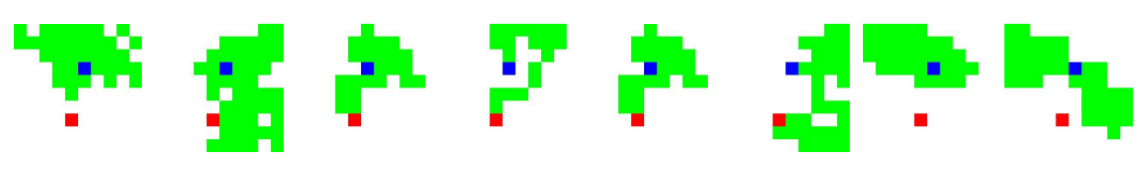
\includegraphics[width=0.7\textwidth]{examples/plan/htm_path_1}
		
		\begin{itemize}
			\item Формирование новых каузальных матриц по данным с сенсоров - модель обучения с подкреплением (агент - среда).
			\item За каждое действие агент получает награду, если он идет кратчайшим путем к конечному положение, то он получит большую награду. 
			\item HCN на простой карте: $\sim 700$ итераций (1 клетка в колонке), $1800$ итераций (с двумя клетками).
			\item Нейронная сеть (2 сверточных слоя и 5 полносвязных) на большой карте: только демонстрирует сходимость процесса обучения. 
		\end{itemize}
		\vspace{-5pt}
		\begin{columns}
			\begin{column}{0.5\textwidth}
				\centering
				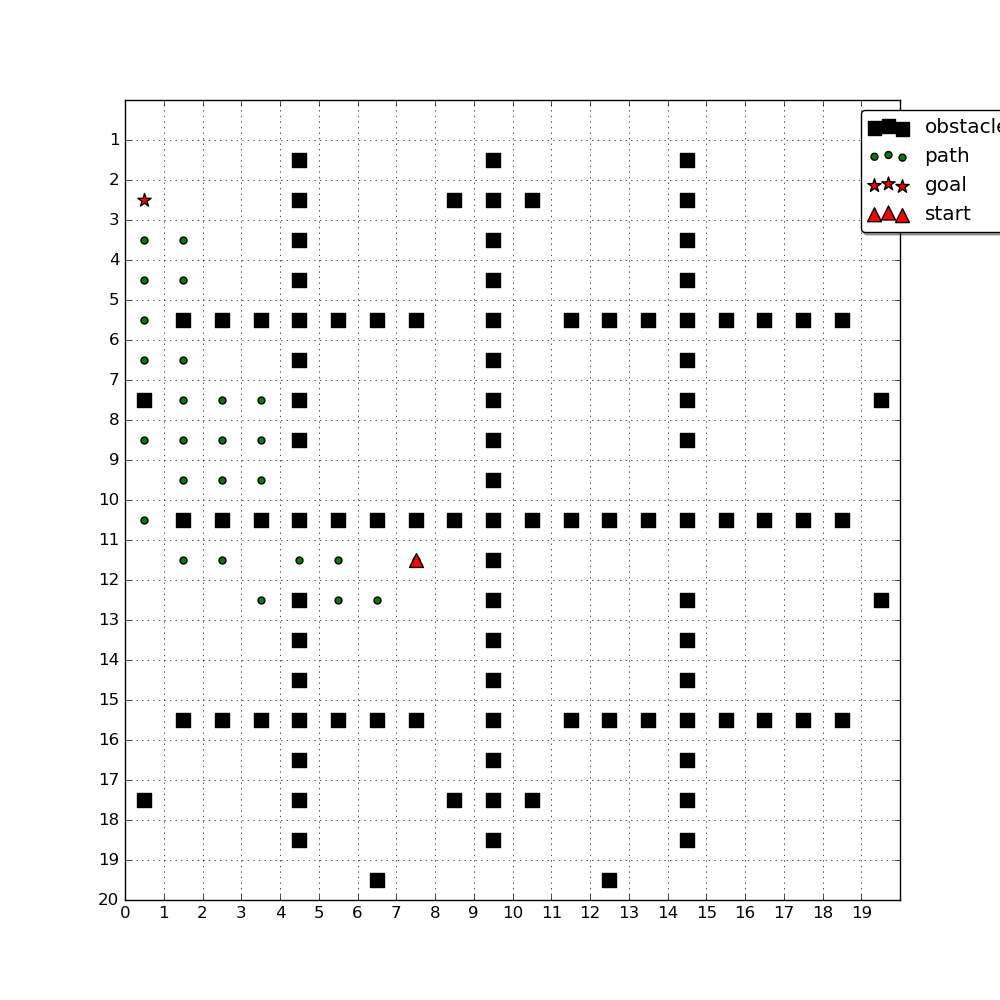
\includegraphics[width=0.4\textwidth]{examples/plan/deeppath_raw}
			\end{column}
			\begin{column}{0.5\textwidth}
				\centering
				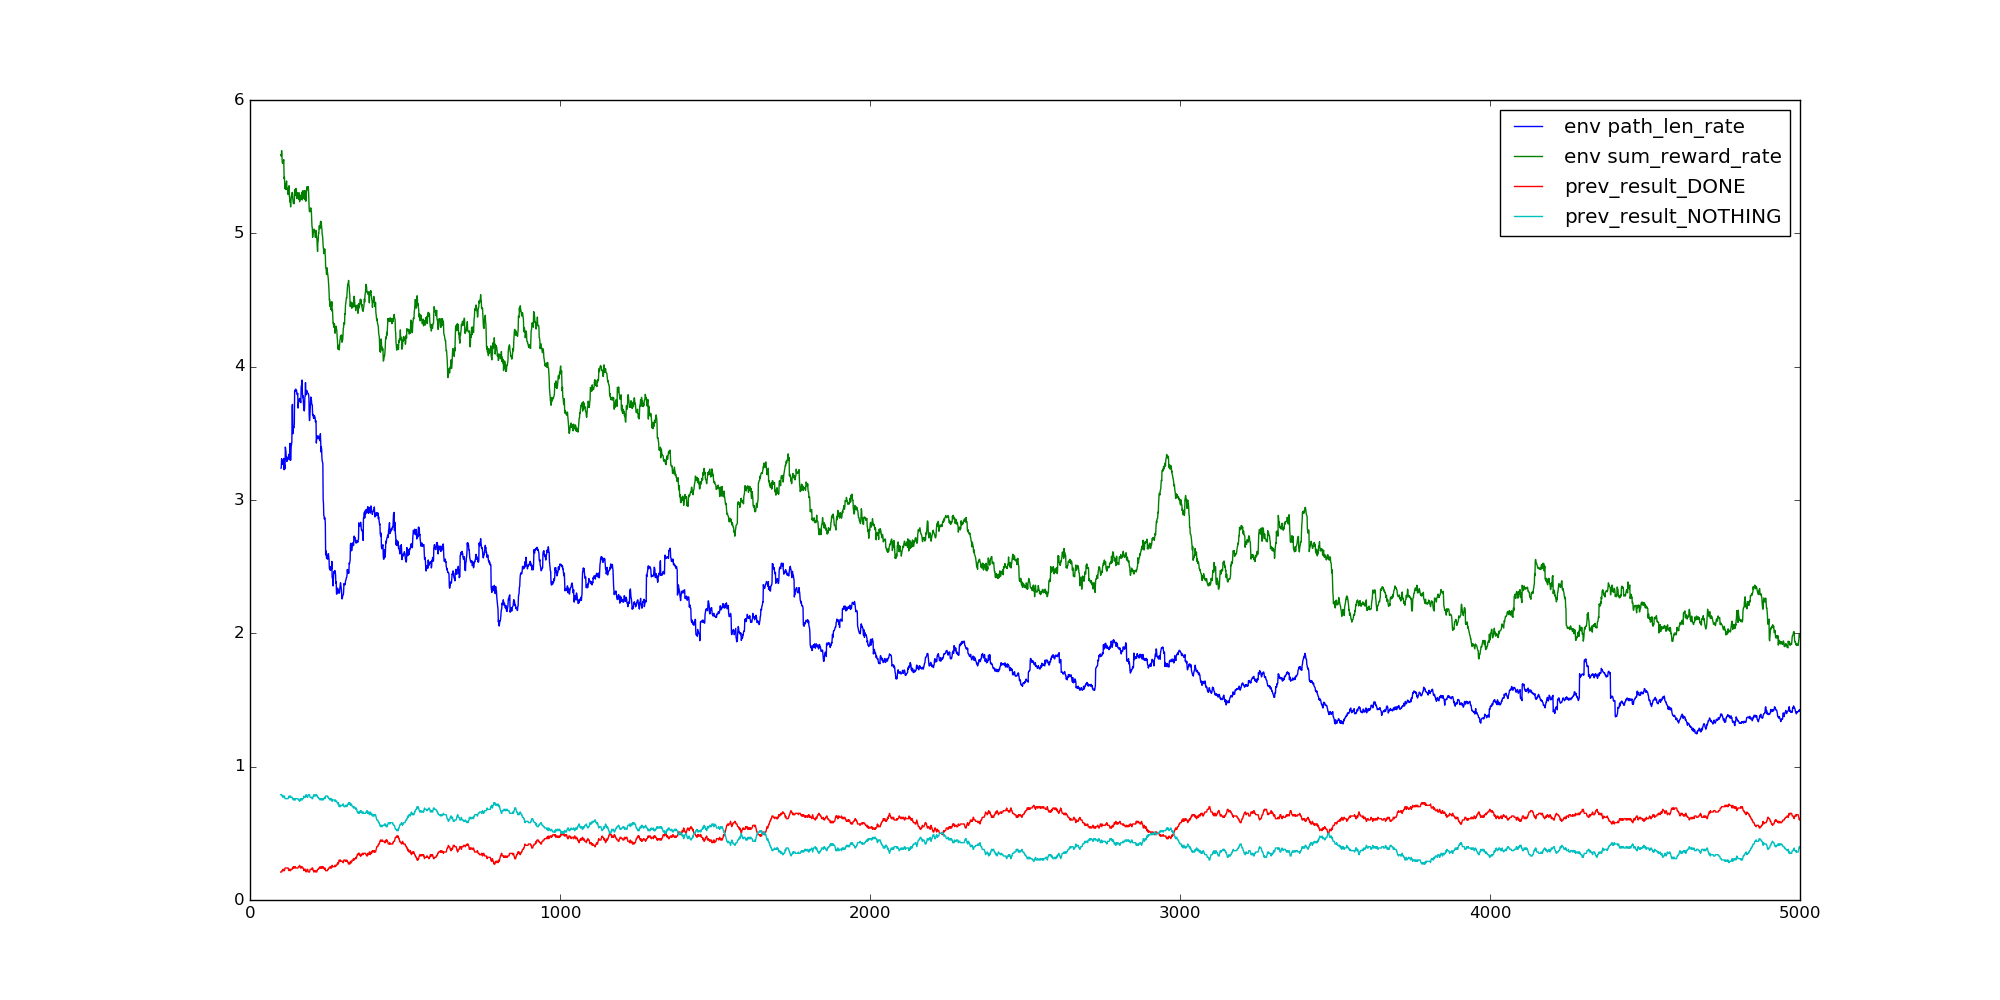
\includegraphics[width=0.9\textwidth]{examples/plan/deeppath_conv_a}
			\end{column}
		\end{columns}
	
	\end{frame}	

	\begin{frame}
		\frametitle{Список публикаций}
		
		\nocite{*}
		\printbibliography[keyword={fulllist}, resetnumbers=true]
	\end{frame}	
				
	\begin{frame}
		\centering
		\Huge
		Спасибо за внимание!
		\normalsize
		\par\bigskip
		\par\bigskip
		\par\bigskip
		pan@isa.ru
		\par\bigskip
		\url{https://github.com/cog-isa/map-planner.git}
	\end{frame}			
\end{document}
	
	
